% Compile with XeLaTeX (needed for Hindi):  xelatex report.tex   (run twice)
% Keep this file next to the .py files and the results/ folder.
\documentclass[12pt,a4paper]{article}
\usepackage[margin=1in]{geometry}
\usepackage{fontspec}
\usepackage{graphicx,float,booktabs,longtable,xcolor,amsmath,listings,tikz}
\usetikzlibrary{arrows.meta,positioning}
\usepackage[hidelinks]{hyperref}
\usepackage{setspace}\onehalfspacing

% Hindi font -- Windows: Nirmala UI | macOS: Kohinoor Devanagari | Linux/Overleaf: Noto Sans Devanagari
\newfontfamily\hindifont[Script=Devanagari]{Nirmala UI}

\newcommand{\todo}[1]{\textcolor{red}{[#1]}}
\newcommand{\safefig}[3]{\begin{figure}[H]\centering
  \IfFileExists{#1}{\includegraphics[width=0.75\textwidth]{#1}}{\fbox{\todo{run scripts to create \detokenize{#1}}}}
  \caption{#2}\label{#3}\end{figure}}
\newcommand{\safeinput}[1]{\IfFileExists{#1}{\input{#1}}{\todo{missing \detokenize{#1}}}}
\newcommand{\codefile}[1]{\IfFileExists{#1}{\lstinputlisting[language=Python,caption={\texttt{\detokenize{#1}}}]{#1}}{\todo{\detokenize{#1} not found}}}
\lstset{basicstyle=\ttfamily\scriptsize,breaklines=true,numbers=left,numberstyle=\tiny,frame=single}

\begin{document}

\begin{titlepage}\centering
{\large B.M.S. Institute of Technology and Management\\ Department of Computer Science and Engineering}\\[1.5cm]
{\Large \textbf{CCA Report -- Natural Language Processing (BCS703A)}}\\[1cm]
{\LARGE \textbf{Machine Translation (English $\rightarrow$ Hindi): Seq2Seq Baseline, MarianMT and Gemini}}\\[1.5cm]
\textbf{Team No.:} \todo{team number}\\[0.5cm]
\begin{tabular}{lll}\toprule \textbf{Name} & \textbf{USN} & \textbf{Roll No.} \\ \midrule
\todo{name 1} & \todo{USN} & \todo{roll} \\ \todo{name 2} & \todo{USN} & \todo{roll} \\ \bottomrule\end{tabular}\\[1.5cm]
\textbf{Faculty:} \todo{faculty name} \qquad Academic Year: \todo{20XX--XX}
\end{titlepage}

\begin{abstract}
This project compares three English-to-Hindi machine translation approaches on the OPUS-100 corpus: a small GRU encoder--decoder
with attention trained from scratch, a pretrained translation tool (MarianMT), and a large language model (Google Gemini) used with zero-shot,
few-shot and chain-of-thought prompts. Text is cleaned, tokenized and analysed with spaCy (POS tags and dependency parse) before training.
All systems are scored on the same test sentences using BLEU, chrF and ROUGE-1 and compared on speed and error types.
The from-scratch model reached BLEU \todo{x}, MarianMT \todo{y} and the best Gemini prompt \todo{z}.
\todo{Add 2--3 sentences with your main conclusion, e.g.\ which system is best and when the small model is still useful.}
\end{abstract}

\tableofcontents\newpage

\section{Introduction and Problem Statement}
\subsection{Background and Domain Context}
Machine translation (MT) automatically converts text from one language to another. Neural MT uses encoder--decoder networks, first with recurrent units
and attention~\cite{bahdanau2015}, later with Transformers~\cite{tiedemann2020}. Large language models can now translate without task-specific training~\cite{brown2020}.
English$\rightarrow$Hindi is challenging because of different word order (SVO vs.\ SOV) and rich morphology.

\subsection{Problem Statement and Task Definition}
Implement machine translation using a Python NLP/translation tool and compare the translation quality with an LLM-based translation approach.
\todo{Replace with the exact CCA statement if different.} \textbf{Input:} an English sentence (3--20 tokens). \textbf{Output:} its Hindi translation (Devanagari).

\subsection{Objectives and Project Scope}
\begin{itemize}
\item Preprocess a parallel corpus and apply POS tagging and dependency parsing.
\item Train and evaluate a Seq2Seq-with-attention baseline.
\item Translate with a pretrained tool (MarianMT) and with Gemini (zero-shot, few-shot, chain-of-thought).
\item Compare quality, speed and errors of all systems.
\end{itemize}

\section{Data Preprocessing and Classical NLP Implementation}
\subsection{Dataset Description and Preparation}
The English--Hindi part of OPUS-100~\cite{zhang2020} (first 30{,}000 pairs, loaded with Hugging Face \texttt{datasets}).
Pairs were kept if both sides have 3--20 tokens; duplicates were removed. Random 80/10/10 split (seed 42).
\begin{table}[H]\centering\safeinput{results/stats.tex}\caption{Dataset statistics.}\end{table}

\subsection{Text Preprocessing Pipeline}
\begin{enumerate}
\item \textbf{Cleaning:} English lowercased, contractions expanded (\emph{can't} $\rightarrow$ \emph{cannot}), characters outside \texttt{a-z0-9 .,?!} removed;
Hindi keeps only Devanagari, digits and punctuation.
\item \textbf{Tokenization:} punctuation split off, then whitespace split (the regex \texttt{\textbackslash w} is avoided because it breaks Hindi words at vowel signs).
\item \textbf{Vocabulary:} built on the training split only; words seen fewer than 2 times become \texttt{<unk>}; special tokens \texttt{<pad>, <sos>, <eos>, <unk>}.
\end{enumerate}

\subsection{Classical NLP and Syntactic Parsing}
spaCy (\texttt{en\_core\_web\_sm})~\cite{honnibal2017} was used for POS tagging (Figure~\ref{fig:pos}) and dependency parsing (Table~\ref{tab:dep}).
\safefig{results/pos_distribution.png}{POS tag distribution on 1000 training sentences.}{fig:pos}
\todo{Comment: which tags dominate and why verbs/nouns matter for translation.}
\begin{table}[H]\centering\safeinput{results/dep_table.tex}\caption{Dependency parse of a sample sentence.}\label{tab:dep}\end{table}
\todo{Comment: English is subject--verb--object, Hindi is subject--object--verb, so the model must reorder words.}

\section{Model Development and Performance Evaluation}
\subsection{Baseline Model Architecture}
A GRU encoder reads the English sentence. A GRU decoder generates Hindi one token at a time; at every step it computes dot-product attention over the
encoder states, concatenates the context vector with its own output, and a linear layer predicts the next word.
\begin{figure}[H]\centering\resizebox{\textwidth}{!}{%
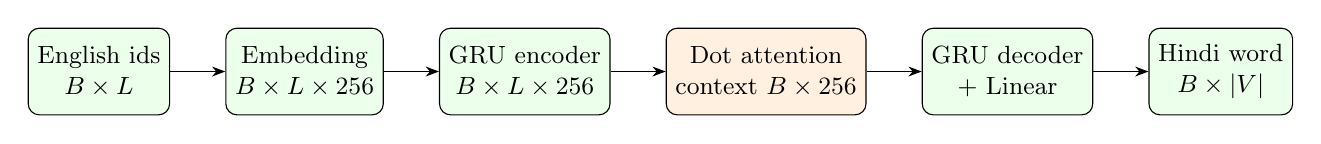
\begin{tikzpicture}[node distance=7mm,box/.style={draw,rounded corners,align=center,minimum height=1.1cm,font=\small,fill=green!8},>=Stealth]
\node[box](a){English ids\\$B\times L$};
\node[box,right=of a](b){Embedding\\$B\times L\times256$};
\node[box,right=of b](c){GRU encoder\\$B\times L\times256$};
\node[box,right=of c,fill=orange!12](d){Dot attention\\context $B\times256$};
\node[box,right=of d](e){GRU decoder\\+ Linear};
\node[box,right=of e](f){Hindi word\\$B\times|V|$};
\draw[->](a)--(b);\draw[->](b)--(c);\draw[->](c)--(d);\draw[->](d)--(e);\draw[->](e)--(f);
\end{tikzpicture}}\caption{Baseline architecture ($B$ = batch, $L$ = source length).}\end{figure}

\subsection{Experimental Setup and Training Details}
Embedding/hidden size 256, batch size 128, 10 epochs, Adam (learning rate $10^{-3}$), cross-entropy loss (padding ignored), dropout 0.3,
gradient clipping 1.0, teacher forcing 0.5, greedy decoding. Best epoch kept by validation loss.
Environment: NVIDIA GeForce RTX 4060 Laptop GPU, Windows, Python 3.10, PyTorch.

\subsection{Performance Evaluation and Results}
Metrics: BLEU (SacreBLEU)~\cite{papineni2002}, chrF~\cite{popovic2015}, ROUGE-1~\cite{lin2004} (own implementation) and perplexity. METEOR is not used because
its standard version does not support Hindi.
\safefig{results/loss_curve.png}{Training and validation loss.}{fig:loss}
\todo{Comment: when validation loss stops improving; any overfitting.}
\begin{table}[H]\centering\safeinput{results/baseline_table.tex}\caption{Baseline results.}\end{table}

\section{LLM-based Implementation and Comparative Analysis}
\subsection{LLM Framework and Setup}
Google Gemini (\texttt{gemini-3.5-flash}) was called through the \texttt{google-genai} Python SDK. MarianMT \texttt{opus-mt-en-hi}~\cite{tiedemann2020}
(beam size 4) is the pretrained translation tool. Both receive the raw English sentence; the baseline receives the cleaned one.
All outputs get the same Hindi normalisation before scoring. Prompts (see Appendix): \textbf{zero-shot} (instruction only), \textbf{few-shot} (3 training examples)
and \textbf{chain-of-thought}~\cite{wei2022} (think about words, order and tense, then give the final line).

\subsection{Comparative Evaluation (Classical vs.\ LLM)}
\begin{table}[H]\centering\small\safeinput{results/results_table.tex}\caption{All systems on the same test sentences.}\end{table}
\safefig{results/comparison_bar.png}{BLEU and chrF per system.}{fig:bar}
\todo{Comment: ranking, effect of the prompt style, speed difference.}

\noindent\textbf{Example outputs.}
{\small\safeinput{results/samples_table.tex}}
\todo{Comment on fluency, meaning and word order in these examples.}

\subsection{Comprehensive Error Analysis}
\textbf{Lexical:} \todo{rare words turned into \texttt{<unk>}/dropped by the baseline; examples}.
\textbf{Syntactic:} \todo{word-order, gender/number agreement, tense errors, repeated words}.
\textbf{Semantic:} \todo{wrong meaning, missing or added content}.
\textbf{Resources:} the baseline is small and fast but needs training; Gemini needs no training but needs internet, has latency, rate limits and sends text to a third party.
\todo{Add measured ms/sentence from the table.}

\section{Conclusion and Future Scope}
\subsection{Summary of Contributions}
We built a preprocessing and parsing pipeline, a Seq2Seq-attention baseline, and compared it with MarianMT and Gemini on English$\rightarrow$Hindi.
\todo{State your findings and when each approach is best.}
\subsection{Future Enhancements}
Subword tokenization (BPE), Transformer baseline, beam search, fine-tuning an open LLM, glossaries/RAG for domain terms, and COMET/BERTScore with human evaluation.

\section{References and Appendix}
\begin{thebibliography}{9}
\bibitem{bahdanau2015} D.\ Bahdanau, K.\ Cho, Y.\ Bengio, ``Neural machine translation by jointly learning to align and translate,'' \emph{ICLR}, 2015.
\bibitem{papineni2002} K.\ Papineni et al., ``BLEU: a method for automatic evaluation of machine translation,'' \emph{ACL}, 2002.
\bibitem{popovic2015} M.\ Popovi\'c, ``chrF: character n-gram F-score for automatic MT evaluation,'' \emph{WMT}, 2015.
\bibitem{lin2004} C.-Y.\ Lin, ``ROUGE: A package for automatic evaluation of summaries,'' \emph{Text Summarization Branches Out}, 2004.
\bibitem{zhang2020} B.\ Zhang et al., ``Improving massively multilingual neural machine translation and zero-shot translation,'' \emph{ACL}, 2020.
\bibitem{tiedemann2020} J.\ Tiedemann, S.\ Thottingal, ``OPUS-MT -- Building open translation services for the world,'' \emph{EAMT}, 2020.
\bibitem{brown2020} T.\ Brown et al., ``Language models are few-shot learners,'' \emph{NeurIPS}, 2020.
\bibitem{wei2022} J.\ Wei et al., ``Chain-of-thought prompting elicits reasoning in large language models,'' \emph{NeurIPS}, 2022.
\bibitem{honnibal2017} M.\ Honnibal, I.\ Montani, ``spaCy 2: Natural language understanding with Bloom embeddings, convolutional neural networks and incremental parsing,'' 2017.
\end{thebibliography}

\appendix
\section*{Appendix A -- Prompts}
\begin{lstlisting}[numbers=none]
ZERO-SHOT: Translate this English sentence into Hindi (Devanagari). Output only the translation.
           English: {sentence}
FEW-SHOT:  Translate English into Hindi (Devanagari). Output only the translation.
           English: {example}  Hindi: {example}  (3 examples)  English: {sentence}  Hindi:
CoT:       Translate this English sentence into Hindi (Devanagari). First think step by step about key words,
           word order and tense. Then end with a last line 'Translation: <Hindi sentence>'.
           English: {sentence}
\end{lstlisting}

\section*{Appendix B -- Code}
\codefile{common.py}
\codefile{prep.py}
\codefile{train.py}
\codefile{translate.py}
\codefile{compare.py}
\end{document}
